\documentclass[twoside]{book}

% Packages required by doxygen
\usepackage{fixltx2e}
\usepackage{calc}
\usepackage{doxygen}
\usepackage{graphicx}
\usepackage[utf8]{inputenc}
\usepackage{makeidx}
\usepackage{multicol}
\usepackage{multirow}
\PassOptionsToPackage{warn}{textcomp}
\usepackage{textcomp}
\usepackage[nointegrals]{wasysym}
\usepackage[table]{xcolor}

% Font selection
\usepackage[T1]{fontenc}
\usepackage{mathptmx}
\usepackage[scaled=.90]{helvet}
\usepackage{courier}
\usepackage{amssymb}
\usepackage{sectsty}
\renewcommand{\familydefault}{\sfdefault}
\allsectionsfont{%
  \fontseries{bc}\selectfont%
  \color{darkgray}%
}
\renewcommand{\DoxyLabelFont}{%
  \fontseries{bc}\selectfont%
  \color{darkgray}%
}
\newcommand{\+}{\discretionary{\mbox{\scriptsize$\hookleftarrow$}}{}{}}

% Page & text layout
\usepackage{geometry}
\geometry{%
  a4paper,%
  top=2.5cm,%
  bottom=2.5cm,%
  left=2.5cm,%
  right=2.5cm%
}
\tolerance=750
\hfuzz=15pt
\hbadness=750
\setlength{\emergencystretch}{15pt}
\setlength{\parindent}{0cm}
\setlength{\parskip}{0.2cm}
\makeatletter
\renewcommand{\paragraph}{%
  \@startsection{paragraph}{4}{0ex}{-1.0ex}{1.0ex}{%
    \normalfont\normalsize\bfseries\SS@parafont%
  }%
}
\renewcommand{\subparagraph}{%
  \@startsection{subparagraph}{5}{0ex}{-1.0ex}{1.0ex}{%
    \normalfont\normalsize\bfseries\SS@subparafont%
  }%
}
\makeatother

% Headers & footers
\usepackage{fancyhdr}
\pagestyle{fancyplain}
\fancyhead[LE]{\fancyplain{}{\bfseries\thepage}}
\fancyhead[CE]{\fancyplain{}{}}
\fancyhead[RE]{\fancyplain{}{\bfseries\leftmark}}
\fancyhead[LO]{\fancyplain{}{\bfseries\rightmark}}
\fancyhead[CO]{\fancyplain{}{}}
\fancyhead[RO]{\fancyplain{}{\bfseries\thepage}}
\fancyfoot[LE]{\fancyplain{}{}}
\fancyfoot[CE]{\fancyplain{}{}}
\fancyfoot[RE]{\fancyplain{}{\bfseries\scriptsize Generated on Sun Dec 20 2015 10\+:53\+:48 for Simulador Rede de Petri (ex12) by Doxygen }}
\fancyfoot[LO]{\fancyplain{}{\bfseries\scriptsize Generated on Sun Dec 20 2015 10\+:53\+:48 for Simulador Rede de Petri (ex12) by Doxygen }}
\fancyfoot[CO]{\fancyplain{}{}}
\fancyfoot[RO]{\fancyplain{}{}}
\renewcommand{\footrulewidth}{0.4pt}
\renewcommand{\chaptermark}[1]{%
  \markboth{#1}{}%
}
\renewcommand{\sectionmark}[1]{%
  \markright{\thesection\ #1}%
}

% Indices & bibliography
\usepackage{natbib}
\usepackage[titles]{tocloft}
\setcounter{tocdepth}{3}
\setcounter{secnumdepth}{5}
\makeindex

% Hyperlinks (required, but should be loaded last)
\usepackage{ifpdf}
\ifpdf
  \usepackage[pdftex,pagebackref=true]{hyperref}
\else
  \usepackage[ps2pdf,pagebackref=true]{hyperref}
\fi
\hypersetup{%
  colorlinks=true,%
  linkcolor=blue,%
  citecolor=blue,%
  unicode%
}

% Custom commands
\newcommand{\clearemptydoublepage}{%
  \newpage{\pagestyle{empty}\cleardoublepage}%
}


%===== C O N T E N T S =====

\begin{document}

% Titlepage & ToC
\hypersetup{pageanchor=false,
             bookmarks=true,
             bookmarksnumbered=true,
             pdfencoding=unicode
            }
\pagenumbering{roman}
\begin{titlepage}
\vspace*{7cm}
\begin{center}%
{\Large Simulador Rede de Petri (ex12) \\[1ex]\large 2.\+0 }\\
\vspace*{1cm}
{\large Generated by Doxygen 1.8.8}\\
\vspace*{0.5cm}
{\small Sun Dec 20 2015 10:53:48}\\
\end{center}
\end{titlepage}
\clearemptydoublepage
\tableofcontents
\clearemptydoublepage
\pagenumbering{arabic}
\hypersetup{pageanchor=true}

%--- Begin generated contents ---
\chapter{Main Page}
\label{index}\hypertarget{index}{}Simulador Rede de Petri Exercício 12 da cadeira de matemática discreta, utilizado como requisito para avaliação final.

Este programa tem como finalidade simular uma R\+E\+D\+E D\+E P\+E\+T\+R\+I, utilizando o conceito de Threads para executar as ações separadamente e utilizando listas lineares.

\begin{DoxyVersion}{Version}
20151219.\+172800 
\end{DoxyVersion}
\begin{DoxyDate}{Date}
2015-\/12-\/19
\end{DoxyDate}
\begin{DoxyAuthor}{Author}
Paulo Vítor Alves Patriota 

João Pedro Pacheco Rodrigues Almeida
\end{DoxyAuthor}
\begin{DoxyParagraph}{Webpage}
$<$\href{http://www.upe.br}{\tt http\+://www.\+upe.\+br}$>$
\end{DoxyParagraph}
\begin{DoxyCopyright}{Copyright}
(c) 2015 
\end{DoxyCopyright}

\chapter{Data Structure Index}
\section{Data Structures}
Here are the data structures with brief descriptions\+:\begin{DoxyCompactList}
\item\contentsline{section}{\hyperlink{structsarcos}{sarcos} \\*
\begin{DoxyItemize}
\item A estrutura sarcos cujo o nome definido foi arcos, irá armazenar as informacoes sobre os arcos da rede de petri 
\end{DoxyItemize}}{\pageref{structsarcos}}{}
\item\contentsline{section}{\hyperlink{structsestados}{sestados} \\*
\begin{DoxyItemize}
\item Estruturas utilizadas para o correto funcionamento do programa 
\end{DoxyItemize}}{\pageref{structsestados}}{}
\item\contentsline{section}{\hyperlink{structstadt}{stadt} \\*
\begin{DoxyItemize}
\item A estrutura stadt cujo o nome definido foi tadt, irá auxiliar o programa na criação das threads 
\end{DoxyItemize}}{\pageref{structstadt}}{}
\item\contentsline{section}{\hyperlink{structstransicoes}{stransicoes} \\*
\begin{DoxyItemize}
\item A estrutura stransicoes cujo o nome definido foi transicoes, irá armazenar as informacoes sobre as transicoes da rede de petri 
\end{DoxyItemize}}{\pageref{structstransicoes}}{}
\end{DoxyCompactList}

\chapter{File Index}
\section{File List}
Here is a list of all documented files with brief descriptions\+:\begin{DoxyCompactList}
\item\contentsline{section}{\hyperlink{ex12_8c}{ex12.\+c} \\*Programa que simula a rede de petri utilizando threads e listas }{\pageref{ex12_8c}}{}
\end{DoxyCompactList}

\chapter{Data Structure Documentation}
\hypertarget{structsarcos}{\section{sarcos Struct Reference}
\label{structsarcos}\index{sarcos@{sarcos}}
}



\begin{DoxyItemize}
\item A estrutura sarcos cujo o nome definido foi arcos, irá armazenar as informacoes sobre os arcos da rede de petri. 
\end{DoxyItemize} 




Collaboration diagram for sarcos\+:\nopagebreak
\begin{figure}[H]
\begin{center}
\leavevmode
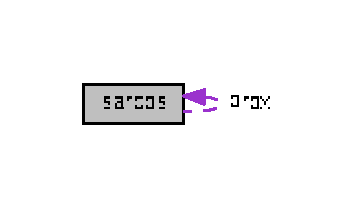
\includegraphics[width=171pt]{structsarcos__coll__graph}
\end{center}
\end{figure}
\subsection*{Data Fields}
\begin{DoxyCompactItemize}
\item 
\hypertarget{structsarcos_a6fcf2f0844e9df8a952c5e320670a78a}{int {\bfseries origem}}\label{structsarcos_a6fcf2f0844e9df8a952c5e320670a78a}

\item 
\hypertarget{structsarcos_aa5d9030bfe6b99fa885afb9ca11a70c4}{int {\bfseries destino}}\label{structsarcos_aa5d9030bfe6b99fa885afb9ca11a70c4}

\item 
\hypertarget{structsarcos_a24fe72482be7db5e96af8eae5316bbb8}{int {\bfseries custo}}\label{structsarcos_a24fe72482be7db5e96af8eae5316bbb8}

\item 
\hypertarget{structsarcos_a9a1c21530791b8ac61f499a2d9b00da6}{struct \hyperlink{structsarcos}{sarcos} $\ast$ {\bfseries prox}}\label{structsarcos_a9a1c21530791b8ac61f499a2d9b00da6}

\end{DoxyCompactItemize}


\subsection{Detailed Description}

\begin{DoxyItemize}
\item A estrutura sarcos cujo o nome definido foi arcos, irá armazenar as informacoes sobre os arcos da rede de petri. 
\end{DoxyItemize}


\begin{DoxyParams}[1]{Parameters}
\mbox{\tt in}  & {\em -\/} & A variavel O\+R\+I\+G\+E\+M do tipo int, irá indicar o ponto de origem da transicao, ou seja, de qual transicao o token irá sair. \\
\hline
\mbox{\tt in}  & {\em -\/} & A variável D\+E\+S\+T\+I\+N\+O do tipo int, irá indicar o ponto de chegada de uma transicao, ou seja, em qual transicao o token irá chegar. \\
\hline
\mbox{\tt in}  & {\em -\/} & A variável C\+U\+S\+T\+O do tipo int, irá indicar o custo da transicao, ou seja, a quantidade de tokens que uma determinada transicao irá enviar. \\
\hline
\mbox{\tt out}  & {\em -\/} & O ponteiro prox aponta para o elemento seguinte da lista. Este ponteiro é uma variável da estrutura stadt, que é a estrutura responsável pelo auxilo na hora de criar as threads. \\
\hline
\end{DoxyParams}


Definition at line 178 of file ex12.\+c.



The documentation for this struct was generated from the following file\+:\begin{DoxyCompactItemize}
\item 
\hyperlink{ex12_8c}{ex12.\+c}\end{DoxyCompactItemize}

\hypertarget{structsestados}{\section{sestados Struct Reference}
\label{structsestados}\index{sestados@{sestados}}
}



\begin{DoxyItemize}
\item Estruturas utilizadas para o correto funcionamento do programa. 
\end{DoxyItemize} 




Collaboration diagram for sestados\+:\nopagebreak
\begin{figure}[H]
\begin{center}
\leavevmode
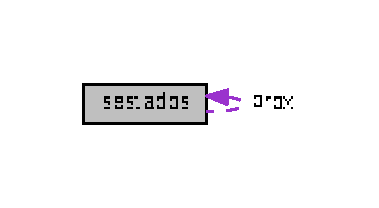
\includegraphics[width=182pt]{structsestados__coll__graph}
\end{center}
\end{figure}
\subsection*{Data Fields}
\begin{DoxyCompactItemize}
\item 
\hypertarget{structsestados_ab1e12f04caa9249050af9140d8bb43ef}{int {\bfseries ne}}\label{structsestados_ab1e12f04caa9249050af9140d8bb43ef}

\item 
\hypertarget{structsestados_a911517ed0c8acbdf708735e8b1027db8}{int {\bfseries nt}}\label{structsestados_a911517ed0c8acbdf708735e8b1027db8}

\item 
\hypertarget{structsestados_a9afdff2fdafac8a7824f0539bbe11003}{struct \hyperlink{structsestados}{sestados} $\ast$ {\bfseries prox}}\label{structsestados_a9afdff2fdafac8a7824f0539bbe11003}

\end{DoxyCompactItemize}


\subsection{Detailed Description}

\begin{DoxyItemize}
\item Estruturas utilizadas para o correto funcionamento do programa. 
\end{DoxyItemize}


\begin{DoxyItemize}
\item A estrutura sestados cujo o nome definido foi estados, irá armazenar as informacoes sobre os estados da rede de petri. 
\begin{DoxyParams}[1]{Parameters}
\mbox{\tt in}  & {\em -\/} & Ne recebe o número de estados. \\
\hline
\mbox{\tt in}  & {\em -\/} & Nt recebe o numero de tokens de cada estado. \\
\hline
\mbox{\tt out}  & {\em -\/} & O ponteiro prox aponta para o elemento seguinte da lista. Este ponteiro também é uma variável da estrutura sestados. \\
\hline
\end{DoxyParams}

\end{DoxyItemize}

Definition at line 145 of file ex12.\+c.



The documentation for this struct was generated from the following file\+:\begin{DoxyCompactItemize}
\item 
\hyperlink{ex12_8c}{ex12.\+c}\end{DoxyCompactItemize}

\hypertarget{structstadt}{\section{stadt Struct Reference}
\label{structstadt}\index{stadt@{stadt}}
}



\begin{DoxyItemize}
\item A estrutura stadt cujo o nome definido foi tadt, irá auxiliar o programa na criação das threads. 
\end{DoxyItemize} 




Collaboration diagram for stadt\+:\nopagebreak
\begin{figure}[H]
\begin{center}
\leavevmode
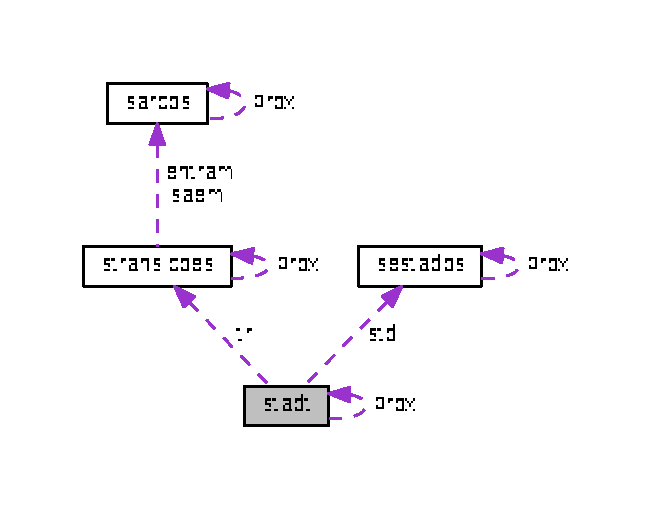
\includegraphics[width=314pt]{structstadt__coll__graph}
\end{center}
\end{figure}
\subsection*{Data Fields}
\begin{DoxyCompactItemize}
\item 
\hypertarget{structstadt_a6b70aec44f3debbafe744148c4d4ecdf}{pthread\+\_\+t {\bfseries nth}}\label{structstadt_a6b70aec44f3debbafe744148c4d4ecdf}

\item 
\hypertarget{structstadt_a9f407187c32ee51a170aad3f1699f042}{struct \hyperlink{structstransicoes}{stransicoes} $\ast$ {\bfseries tr}}\label{structstadt_a9f407187c32ee51a170aad3f1699f042}

\item 
\hypertarget{structstadt_a4d45b2162d0eef245b092ef52da98e5a}{struct \hyperlink{structsestados}{sestados} $\ast$ {\bfseries std}}\label{structstadt_a4d45b2162d0eef245b092ef52da98e5a}

\item 
\hypertarget{structstadt_a3d7dd6a9dcaeab4f8c346ae48437dc35}{struct \hyperlink{structstadt}{stadt} $\ast$ {\bfseries prox}}\label{structstadt_a3d7dd6a9dcaeab4f8c346ae48437dc35}

\end{DoxyCompactItemize}


\subsection{Detailed Description}

\begin{DoxyItemize}
\item A estrutura stadt cujo o nome definido foi tadt, irá auxiliar o programa na criação das threads. 
\end{DoxyItemize}

Definition at line 189 of file ex12.\+c.



The documentation for this struct was generated from the following file\+:\begin{DoxyCompactItemize}
\item 
\hyperlink{ex12_8c}{ex12.\+c}\end{DoxyCompactItemize}

\hypertarget{structstransicoes}{\section{stransicoes Struct Reference}
\label{structstransicoes}\index{stransicoes@{stransicoes}}
}



\begin{DoxyItemize}
\item A estrutura stransicoes cujo o nome definido foi transicoes, irá armazenar as informacoes sobre as transicoes da rede de petri. 
\end{DoxyItemize} 




Collaboration diagram for stransicoes\+:\nopagebreak
\begin{figure}[H]
\begin{center}
\leavevmode
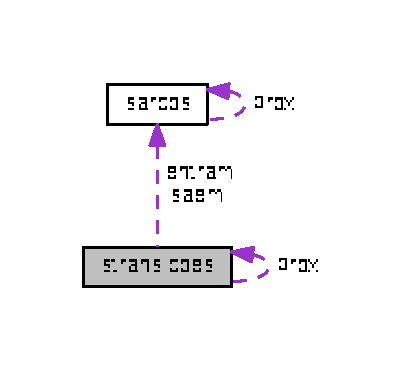
\includegraphics[width=194pt]{structstransicoes__coll__graph}
\end{center}
\end{figure}
\subsection*{Data Fields}
\begin{DoxyCompactItemize}
\item 
\hypertarget{structstransicoes_ae97cbc2aefd98500d0926dcee3dc7ba9}{int {\bfseries ntr}}\label{structstransicoes_ae97cbc2aefd98500d0926dcee3dc7ba9}

\item 
\hypertarget{structstransicoes_a9b6d3aa4b419f4d1def1fd28bd056d6c}{struct \hyperlink{structstransicoes}{stransicoes} $\ast$ {\bfseries prox}}\label{structstransicoes_a9b6d3aa4b419f4d1def1fd28bd056d6c}

\item 
\hypertarget{structstransicoes_a45642aa4189a4c998f2cb6ba0bfbee28}{struct \hyperlink{structsarcos}{sarcos} $\ast$ {\bfseries entram}}\label{structstransicoes_a45642aa4189a4c998f2cb6ba0bfbee28}

\item 
\hypertarget{structstransicoes_a9dc5695ede661e803acfade92ed9f34d}{struct \hyperlink{structsarcos}{sarcos} $\ast$ {\bfseries saem}}\label{structstransicoes_a9dc5695ede661e803acfade92ed9f34d}

\end{DoxyCompactItemize}


\subsection{Detailed Description}

\begin{DoxyItemize}
\item A estrutura stransicoes cujo o nome definido foi transicoes, irá armazenar as informacoes sobre as transicoes da rede de petri. 
\end{DoxyItemize}


\begin{DoxyParams}[1]{Parameters}
\mbox{\tt in}  & {\em -\/} & N\+T\+R recebe o número de transicoes do arquivo de leitura. \\
\hline
\mbox{\tt out}  & {\em -\/} & O ponteiro prox aponta para o elemento seguinte da lista. Este ponteiro também é uma variável da estrutura stransicoes. \\
\hline
\mbox{\tt out}  & {\em -\/} & O ponteiro entram é um ponteiro de estrutura sarcos e este ponteiro é responsavel por armazenar a quantidade de arcos que entram na respectiva transicao. \\
\hline
\mbox{\tt out}  & {\em -\/} & O ponteiro saem é um ponteiro de estrutura sarcos e este ponteiro é responsável por armazenar a quantidade de arcos que saem da respectiva transicao. \\
\hline
\end{DoxyParams}


Definition at line 160 of file ex12.\+c.



The documentation for this struct was generated from the following file\+:\begin{DoxyCompactItemize}
\item 
\hyperlink{ex12_8c}{ex12.\+c}\end{DoxyCompactItemize}

\chapter{File Documentation}
\hypertarget{ex12_8c}{\section{ex12.\+c File Reference}
\label{ex12_8c}\index{ex12.\+c@{ex12.\+c}}
}


Programa que simula a rede de petri utilizando threads e listas.  


{\ttfamily \#include $<$stdio.\+h$>$}\\*
{\ttfamily \#include $<$pthread.\+h$>$}\\*
{\ttfamily \#include $<$stdlib.\+h$>$}\\*
{\ttfamily \#include $<$allegro.\+h$>$}\\*
{\ttfamily \#include $<$math.\+h$>$}\\*
Include dependency graph for ex12.\+c\+:\nopagebreak
\begin{figure}[H]
\begin{center}
\leavevmode
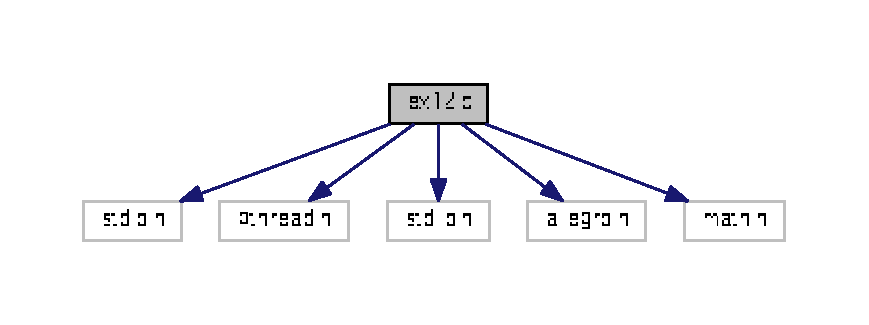
\includegraphics[width=350pt]{ex12_8c__incl}
\end{center}
\end{figure}
\subsection*{Data Structures}
\begin{DoxyCompactItemize}
\item 
struct \hyperlink{structsestados}{sestados}
\begin{DoxyCompactList}\small\item\em 
\begin{DoxyItemize}
\item Estruturas utilizadas para o correto funcionamento do programa. 
\end{DoxyItemize}\end{DoxyCompactList}\item 
struct \hyperlink{structstransicoes}{stransicoes}
\begin{DoxyCompactList}\small\item\em 
\begin{DoxyItemize}
\item A estrutura stransicoes cujo o nome definido foi transicoes, irá armazenar as informacoes sobre as transicoes da rede de petri. 
\end{DoxyItemize}\end{DoxyCompactList}\item 
struct \hyperlink{structsarcos}{sarcos}
\begin{DoxyCompactList}\small\item\em 
\begin{DoxyItemize}
\item A estrutura sarcos cujo o nome definido foi arcos, irá armazenar as informacoes sobre os arcos da rede de petri. 
\end{DoxyItemize}\end{DoxyCompactList}\item 
struct \hyperlink{structstadt}{stadt}
\begin{DoxyCompactList}\small\item\em 
\begin{DoxyItemize}
\item A estrutura stadt cujo o nome definido foi tadt, irá auxiliar o programa na criação das threads. 
\end{DoxyItemize}\end{DoxyCompactList}\end{DoxyCompactItemize}
\subsection*{Macros}
\begin{DoxyCompactItemize}
\item 
\hypertarget{ex12_8c_a8879e1afa8a98a473966caa2eaaf326f}{\#define \hyperlink{ex12_8c_a8879e1afa8a98a473966caa2eaaf326f}{I\+T\+E\+R\+A\+C\+O\+E\+S}~10000}\label{ex12_8c_a8879e1afa8a98a473966caa2eaaf326f}

\begin{DoxyCompactList}\small\item\em 
\begin{DoxyItemize}
\item Quantidade de I\+N\+T\+E\+R\+AÇÕ\+E\+S 
\end{DoxyItemize}\end{DoxyCompactList}\item 
\hypertarget{ex12_8c_ad72dbcf6d0153db1b8d8a58001feed83}{\#define \hyperlink{ex12_8c_ad72dbcf6d0153db1b8d8a58001feed83}{D\+E\+B\+U\+G}~0}\label{ex12_8c_ad72dbcf6d0153db1b8d8a58001feed83}

\begin{DoxyCompactList}\small\item\em 
\begin{DoxyItemize}
\item Define para ativar o D\+E\+B\+U\+G do código. 
\end{DoxyItemize}\end{DoxyCompactList}\item 
\hypertarget{ex12_8c_a3fa02c0d4875f25146e01888e683baaa}{\#define \hyperlink{ex12_8c_a3fa02c0d4875f25146e01888e683baaa}{I\+M\+A\+G\+E\+N\+A\+M\+E}~\char`\"{}ex12.\+bmp\char`\"{} /$\ast$$\ast$Nome do arquivo que sera gerado pelo allegro$\ast$/}\label{ex12_8c_a3fa02c0d4875f25146e01888e683baaa}

\begin{DoxyCompactList}\small\item\em 
\begin{DoxyItemize}
\item Este define foi utilizado para padronizar a saida do arquivo de imagem. 
\end{DoxyItemize}\end{DoxyCompactList}\item 
\hypertarget{ex12_8c_a564a8a1173bd4fb63c4f3a1903143e6a}{\#define \hyperlink{ex12_8c_a564a8a1173bd4fb63c4f3a1903143e6a}{C\+O\+R\+B\+R\+A\+N\+C\+O}~(makecol(255,255,255))}\label{ex12_8c_a564a8a1173bd4fb63c4f3a1903143e6a}

\begin{DoxyCompactList}\small\item\em 
\begin{DoxyItemize}
\item Defines para facilitar o uso da cor branca no allegro. 
\end{DoxyItemize}\end{DoxyCompactList}\item 
\hypertarget{ex12_8c_aaa9af825d3a4f75b40c0403bd37c55bd}{\#define \hyperlink{ex12_8c_aaa9af825d3a4f75b40c0403bd37c55bd}{C\+O\+R\+P\+R\+E\+T\+O}~1}\label{ex12_8c_aaa9af825d3a4f75b40c0403bd37c55bd}

\begin{DoxyCompactList}\small\item\em 
\begin{DoxyItemize}
\item Defines para facilitar o uso da cor preta no allegro. 
\end{DoxyItemize}\end{DoxyCompactList}\item 
\hypertarget{ex12_8c_a6ba7276f7e11d0099ad5386922bfa495}{\#define \hyperlink{ex12_8c_a6ba7276f7e11d0099ad5386922bfa495}{C\+O\+R\+C\+I\+N\+Z\+A}~(makecol(160,160,160))}\label{ex12_8c_a6ba7276f7e11d0099ad5386922bfa495}

\begin{DoxyCompactList}\small\item\em 
\begin{DoxyItemize}
\item Defines para facilitar o uso da cor cinza no allegro. 
\end{DoxyItemize}\end{DoxyCompactList}\item 
\hypertarget{ex12_8c_a70d9bb57e73b641e6394d1a743d4d891}{\#define \hyperlink{ex12_8c_a70d9bb57e73b641e6394d1a743d4d891}{C\+O\+R\+A\+Z\+U\+L}~(makecol(0, 0, 255))}\label{ex12_8c_a70d9bb57e73b641e6394d1a743d4d891}

\begin{DoxyCompactList}\small\item\em 
\begin{DoxyItemize}
\item Defines para facilitar o uso da cor azul no allegro. 
\end{DoxyItemize}\end{DoxyCompactList}\item 
\hypertarget{ex12_8c_ad7dde6e35154225591228222edb21c1b}{\#define \hyperlink{ex12_8c_ad7dde6e35154225591228222edb21c1b}{C\+O\+R\+V\+E\+R\+D\+E}~(makecol(0, 255, 0))}\label{ex12_8c_ad7dde6e35154225591228222edb21c1b}

\begin{DoxyCompactList}\small\item\em 
\begin{DoxyItemize}
\item Defines para facilitar o uso da cor verde no allegro. 
\end{DoxyItemize}\end{DoxyCompactList}\item 
\hypertarget{ex12_8c_a70bb1aad71a6f756c61983e9fa967737}{\#define \hyperlink{ex12_8c_a70bb1aad71a6f756c61983e9fa967737}{C\+O\+R\+A\+M\+A\+R\+E\+L\+O}~(makecol(255,255,100))}\label{ex12_8c_a70bb1aad71a6f756c61983e9fa967737}

\begin{DoxyCompactList}\small\item\em 
\begin{DoxyItemize}
\item Defines para facilitar o uso da cor amarela no allegro. 
\end{DoxyItemize}\end{DoxyCompactList}\item 
\hypertarget{ex12_8c_a0e2857429e52d86533c9fcc6b7e92bfb}{\#define \hyperlink{ex12_8c_a0e2857429e52d86533c9fcc6b7e92bfb}{C\+O\+R\+V\+E\+R\+M\+E\+L\+H\+O}~(makecol(255, 0, 0))}\label{ex12_8c_a0e2857429e52d86533c9fcc6b7e92bfb}

\begin{DoxyCompactList}\small\item\em 
\begin{DoxyItemize}
\item Defines para facilitar o uso da cor vermelha no allegro. 
\end{DoxyItemize}\end{DoxyCompactList}\item 
\hypertarget{ex12_8c_a207fd5507206d307cd63f95374fcd00d}{\#define \hyperlink{ex12_8c_a207fd5507206d307cd63f95374fcd00d}{X}~640 /$\ast$$\ast$Definicao do tamanho X da tela $\ast$/}\label{ex12_8c_a207fd5507206d307cd63f95374fcd00d}

\begin{DoxyCompactList}\small\item\em 
\begin{DoxyItemize}
\item Defines que informam qual o tamanho da tela horizontalmente a serutilizada pelo allegro. 
\end{DoxyItemize}\end{DoxyCompactList}\item 
\hypertarget{ex12_8c_a798e4073d613ca5ba9618e1b3253df14}{\#define \hyperlink{ex12_8c_a798e4073d613ca5ba9618e1b3253df14}{Y}~480 /$\ast$$\ast$Definicao do tamanho Y da tela $\ast$/}\label{ex12_8c_a798e4073d613ca5ba9618e1b3253df14}

\begin{DoxyCompactList}\small\item\em 
\begin{DoxyItemize}
\item Defines que informa qual o tamanho da tela verticalmente a ser utilizada pelo allegro. 
\end{DoxyItemize}\end{DoxyCompactList}\item 
\hypertarget{ex12_8c_afbdf6aaa9dc9536814753a2676ae503e}{\#define \hyperlink{ex12_8c_afbdf6aaa9dc9536814753a2676ae503e}{X\+Centro}~\hyperlink{ex12_8c_a207fd5507206d307cd63f95374fcd00d}{X}/2.\+0 /$\ast$$\ast$Definicao do centro da tela da coordenada \hyperlink{ex12_8c_a207fd5507206d307cd63f95374fcd00d}{X}$\ast$/}\label{ex12_8c_afbdf6aaa9dc9536814753a2676ae503e}

\begin{DoxyCompactList}\small\item\em 
\begin{DoxyItemize}
\item Defines que dizem qual é o centro da tela horizontal baseado no valor de X. 
\end{DoxyItemize}\end{DoxyCompactList}\item 
\hypertarget{ex12_8c_a56ca31f80a4aa2287e297e7f9f2530ae}{\#define \hyperlink{ex12_8c_a56ca31f80a4aa2287e297e7f9f2530ae}{Y\+Centro}~\hyperlink{ex12_8c_a798e4073d613ca5ba9618e1b3253df14}{Y}/2.\+0 /$\ast$$\ast$Definicao do centro da tela da coordenada \hyperlink{ex12_8c_a798e4073d613ca5ba9618e1b3253df14}{Y}$\ast$/}\label{ex12_8c_a56ca31f80a4aa2287e297e7f9f2530ae}

\begin{DoxyCompactList}\small\item\em 
\begin{DoxyItemize}
\item Defines que dizem qual é o centro da tela vertical baseado no valor de Y. 
\end{DoxyItemize}\end{DoxyCompactList}\end{DoxyCompactItemize}
\subsection*{Typedefs}
\begin{DoxyCompactItemize}
\item 
typedef struct \hyperlink{structsestados}{sestados} \hyperlink{ex12_8c_a7d78c1f6e437102f3a49d626fe1d3e6e}{estados}
\begin{DoxyCompactList}\small\item\em 
\begin{DoxyItemize}
\item Estruturas utilizadas para o correto funcionamento do programa. 
\end{DoxyItemize}\end{DoxyCompactList}\item 
typedef struct \hyperlink{structstransicoes}{stransicoes} \hyperlink{ex12_8c_af57cd5194722cb8ac16b2dfa9c6e2d8b}{transicoes}
\begin{DoxyCompactList}\small\item\em 
\begin{DoxyItemize}
\item A estrutura stransicoes cujo o nome definido foi transicoes, irá armazenar as informacoes sobre as transicoes da rede de petri. 
\end{DoxyItemize}\end{DoxyCompactList}\item 
typedef struct \hyperlink{structsarcos}{sarcos} \hyperlink{ex12_8c_a3e52f48190690b34117c195de9726cbb}{arcos}
\begin{DoxyCompactList}\small\item\em 
\begin{DoxyItemize}
\item A estrutura sarcos cujo o nome definido foi arcos, irá armazenar as informacoes sobre os arcos da rede de petri. 
\end{DoxyItemize}\end{DoxyCompactList}\item 
\hypertarget{ex12_8c_a963ca2e9e56ad353bdb6b3066d86f9fd}{typedef struct \hyperlink{structstadt}{stadt} \hyperlink{ex12_8c_a963ca2e9e56ad353bdb6b3066d86f9fd}{tadt}}\label{ex12_8c_a963ca2e9e56ad353bdb6b3066d86f9fd}

\begin{DoxyCompactList}\small\item\em 
\begin{DoxyItemize}
\item A estrutura stadt cujo o nome definido foi tadt, irá auxiliar o programa na criação das threads. 
\end{DoxyItemize}\end{DoxyCompactList}\end{DoxyCompactItemize}
\subsection*{Functions}
\begin{DoxyCompactItemize}
\item 
void \hyperlink{ex12_8c_ab01a986d269fe217ffe938d7e9f3c21c}{gerar\+\_\+entrada} (\hyperlink{ex12_8c_a7d78c1f6e437102f3a49d626fe1d3e6e}{estados} $\ast$$\ast$p\+\_\+estados, \hyperlink{ex12_8c_af57cd5194722cb8ac16b2dfa9c6e2d8b}{transicoes} $\ast$$\ast$p\+\_\+transicoes)
\begin{DoxyCompactList}\small\item\em 
\begin{DoxyItemize}
\item Declaração dos protótipos das funcoes que serão utilizadas para simular a rede de petri. 
\end{DoxyItemize}\end{DoxyCompactList}\item 
void \hyperlink{ex12_8c_a3ed0b3b6a46fa2adc642631b338c29a8}{criar\+\_\+threads} (\hyperlink{ex12_8c_a963ca2e9e56ad353bdb6b3066d86f9fd}{tadt} $\ast$$\ast$p\+\_\+threads, \hyperlink{ex12_8c_af57cd5194722cb8ac16b2dfa9c6e2d8b}{transicoes} $\ast$p\+\_\+transicoes, \hyperlink{ex12_8c_a7d78c1f6e437102f3a49d626fe1d3e6e}{estados} $\ast$p\+\_\+estados)
\begin{DoxyCompactList}\small\item\em 
\begin{DoxyItemize}
\item A funcao criar threads é responsável por criar as threads que iram executar o paralelismo do programa. 
\end{DoxyItemize}\end{DoxyCompactList}\item 
void \hyperlink{ex12_8c_a0c0a5050731aa76819931f0de3e22e67}{espera\+\_\+threads} (\hyperlink{ex12_8c_a963ca2e9e56ad353bdb6b3066d86f9fd}{tadt} $\ast$p\+\_\+threads)
\begin{DoxyCompactList}\small\item\em 
\begin{DoxyItemize}
\item A funcao espera\+\_\+threads tem como finalidade esperar que as threads retornem o status de concluidas. 
\end{DoxyItemize}\end{DoxyCompactList}\item 
void $\ast$ \hyperlink{ex12_8c_a83969662b72a8b75daa3984300e945d8}{roda\+\_\+thread} (void $\ast$dados)
\begin{DoxyCompactList}\small\item\em 
\begin{DoxyItemize}
\item A funcao roda thread é a funcao responsável por rodar as threas que foram criadas na funcao criar\+\_\+threads. 
\end{DoxyItemize}\end{DoxyCompactList}\item 
void \hyperlink{ex12_8c_ad3472f68895f18f39d472c23438cbec9}{criar\+\_\+estados} (\hyperlink{ex12_8c_a7d78c1f6e437102f3a49d626fe1d3e6e}{estados} $\ast$$\ast$p\+\_\+estados, int num)
\begin{DoxyCompactList}\small\item\em 
\begin{DoxyItemize}
\item A funcao criar\+\_\+estados, tem como finalidade criar a quantidade de estados que foram lidos a partir da entrada dos arquivos de textos que foram disponibilizados. 
\end{DoxyItemize}\end{DoxyCompactList}\item 
void \hyperlink{ex12_8c_ab6899028256c5ab21c9632d795702571}{criar\+\_\+transicoes} (\hyperlink{ex12_8c_af57cd5194722cb8ac16b2dfa9c6e2d8b}{transicoes} $\ast$$\ast$p\+\_\+transicoes, \hyperlink{ex12_8c_a3e52f48190690b34117c195de9726cbb}{arcos} $\ast$$\ast$p\+\_\+arcos, int a1, int a2, int num)
\begin{DoxyCompactList}\small\item\em 
\begin{DoxyItemize}
\item A funcao criar transicoes é a responsável por criar todas as transicoes necessárias para o correto funcionamento do programa. 
\end{DoxyItemize}\end{DoxyCompactList}\item 
void \hyperlink{ex12_8c_a69f1768f60ef611e0434476b875b909c}{gerar\+\_\+imagem} (\hyperlink{ex12_8c_af57cd5194722cb8ac16b2dfa9c6e2d8b}{transicoes} $\ast$p\+\_\+transicoes)
\begin{DoxyCompactList}\small\item\em 
\begin{DoxyItemize}
\item A funcao gerar\+\_\+imagem será a funcao responsavel por criar a imagem ex12.\+bmp. 
\end{DoxyItemize}\end{DoxyCompactList}\item 
void \hyperlink{ex12_8c_a9ea1b67e3dd2b2218118db0c14a4ff34}{desenha\+\_\+estados} (B\+I\+T\+M\+A\+P $\ast$buff)
\begin{DoxyCompactList}\small\item\em 
\begin{DoxyItemize}
\item A função desenha\+\_\+estados, é a função responsável por pegar a quantidade de estados que foram lidos dos arquivos de textos fornecidos e através de um código matemático, distribuir os estados pelo tamanho da tela. 
\end{DoxyItemize}\end{DoxyCompactList}\item 
void \hyperlink{ex12_8c_a2218e404fb2ec9dd352610badd5239c4}{desenha\+\_\+transicoes} (B\+I\+T\+M\+A\+P $\ast$buff, \hyperlink{ex12_8c_af57cd5194722cb8ac16b2dfa9c6e2d8b}{transicoes} $\ast$p\+\_\+transicoes)
\begin{DoxyCompactList}\small\item\em 
\begin{DoxyItemize}
\item A função desenha\+\_\+transicoes, tem como finalidade desenhar a quantidade de transicoes que foram armazenadas na variavel T\+R após ter sido lida pelos arquivos de texto e assim como a funcao desenha\+\_\+estados, ao final retornará para a funcao gerar\+\_\+imagem, onde será criada a imagem ex12.\+bmp com as transições. 
\end{DoxyItemize}\end{DoxyCompactList}\item 
void \hyperlink{ex12_8c_a93fe8b90c69f52c49c86ccc1d6df7e29}{desenha\+\_\+arcos} (int qo, int qf, B\+I\+T\+M\+A\+P $\ast$buff, int k, int c, int flag)
\begin{DoxyCompactList}\small\item\em 
\begin{DoxyItemize}
\item A funcao desenha\+\_\+arcos tem como finalidade desenhar os arcos que saem dos estados e tem destino nas transicoes e desenhar os arcos que saem das transicoes e tem destino dos estados. 
\end{DoxyItemize}\end{DoxyCompactList}\item 
\hyperlink{ex12_8c_a3e52f48190690b34117c195de9726cbb}{arcos} $\ast$ \hyperlink{ex12_8c_acccd6bffb1caa195b998b151ff7cafce}{retirar\+\_\+arco} (\hyperlink{ex12_8c_a3e52f48190690b34117c195de9726cbb}{arcos} $\ast$$\ast$p\+\_\+arco)
\begin{DoxyCompactList}\small\item\em 
\begin{DoxyItemize}
\item A funcao $\ast$retirar\+\_\+arco é uma função que só é utilizada caso se tenha a intenção ou seja necessário remover um determinado arco. 
\end{DoxyItemize}\end{DoxyCompactList}\item 
void \hyperlink{ex12_8c_afe6e8ec84f7d12cdfcd258f51ef7f7e5}{transferir\+\_\+arco} (\hyperlink{ex12_8c_a3e52f48190690b34117c195de9726cbb}{arcos} $\ast$$\ast$p\+\_\+arco, \hyperlink{ex12_8c_af57cd5194722cb8ac16b2dfa9c6e2d8b}{transicoes} $\ast$p\+\_\+transicao, int a1, int a2)
\begin{DoxyCompactList}\small\item\em 
\begin{DoxyItemize}
\item A funcao transferir arcos tem como finalidade fazer a ligação correta entre os arcos e as transicoes. 
\end{DoxyItemize}\end{DoxyCompactList}\item 
void \hyperlink{ex12_8c_ab52c2d9ac8f7f64221f18ded36d29342}{criar\+\_\+arcos} (\hyperlink{ex12_8c_a3e52f48190690b34117c195de9726cbb}{arcos} $\ast$$\ast$p\+\_\+arcos, int a1, int a2)
\begin{DoxyCompactList}\small\item\em 
\begin{DoxyItemize}
\item A funcao criar arcos é a responsável por criar todos os arcos necessárias para o correto funcionamento do programa. 
\end{DoxyItemize}\end{DoxyCompactList}\item 
void \hyperlink{ex12_8c_a3a6d8dfce1151d4e4235e56875dede10}{relacionar\+\_\+tokens} (\hyperlink{ex12_8c_a7d78c1f6e437102f3a49d626fe1d3e6e}{estados} $\ast$p\+\_\+estados, int num)
\begin{DoxyCompactList}\small\item\em 
\begin{DoxyItemize}
\item A funcao relacionar tokens tem como finalidade relacionar a quantidade de estados com os seus respectivos tokens, ou seja, essa funcao vai inicializar os estados, colocando a quantidade de tokens necessárias a partir da leitura dos arquivos de textos disponibilizados. 
\end{DoxyItemize}\end{DoxyCompactList}\item 
\hyperlink{ex12_8c_a7d78c1f6e437102f3a49d626fe1d3e6e}{estados} $\ast$ \hyperlink{ex12_8c_a9c823955799d7a72079b22b00cff392a}{procurar\+\_\+estado} (\hyperlink{ex12_8c_a7d78c1f6e437102f3a49d626fe1d3e6e}{estados} $\ast$p\+\_\+estados, int num)
\begin{DoxyCompactList}\small\item\em 
\begin{DoxyItemize}
\item A funcao procurar estados vai procurar um determinado estado dentro da lista de estados. 
\end{DoxyItemize}\end{DoxyCompactList}\item 
\hyperlink{ex12_8c_af57cd5194722cb8ac16b2dfa9c6e2d8b}{transicoes} $\ast$ \hyperlink{ex12_8c_ad8bed4f2b548117dc7b62b139317a4e0}{procurar\+\_\+transicao} (\hyperlink{ex12_8c_af57cd5194722cb8ac16b2dfa9c6e2d8b}{transicoes} $\ast$p\+\_\+transicoes, int num)
\begin{DoxyCompactList}\small\item\em 
\begin{DoxyItemize}
\item A funcao procurar transicoes vai procurar uma determinada transicao dentro da lista de transicoes. 
\end{DoxyItemize}\end{DoxyCompactList}\item 
void \hyperlink{ex12_8c_ae315c788a512451cf89281dbbaae1f5f}{debug} (\hyperlink{ex12_8c_a7d78c1f6e437102f3a49d626fe1d3e6e}{estados} $\ast$p\+\_\+estados, \hyperlink{ex12_8c_af57cd5194722cb8ac16b2dfa9c6e2d8b}{transicoes} $\ast$p\+\_\+transicoes)
\begin{DoxyCompactList}\small\item\em 
\begin{DoxyItemize}
\item A funcao D\+E\+B\+U\+G tem como finalidade mostrar um status atual do funcionamento do programa. 
\end{DoxyItemize}\end{DoxyCompactList}\item 
float \hyperlink{ex12_8c_af4699181d7bf8a6ccce6902827c9b975}{arctan} (float x1, float y1, float x2, float y2)
\begin{DoxyCompactList}\small\item\em 
\begin{DoxyItemize}
\item A funcao arctan é a responsavel por fazer as ligacoes corretas dos arcos para os estados ou transicoes, fazendo com que saiam dos centros dos estados e possam chegar nos centros das transicoes ou saindo dos centro das transicoes para chegarem ao centro dos estados. 
\end{DoxyItemize}\end{DoxyCompactList}\item 
float \hyperlink{ex12_8c_adb4877932ec102678fc7b2e07b5ac653}{lcos} (float x1, float y1, float x2, float y2)
\begin{DoxyCompactList}\small\item\em 
\begin{DoxyItemize}
\item A funcao lcos é a responsavel por garantir o posicionamento correto dos arcos com os respectivos centros das transicoes e dos estados. 
\end{DoxyItemize}\end{DoxyCompactList}\item 
float \hyperlink{ex12_8c_a648c3d8c98be97e55642a0a3adc9c82e}{lsin} (float x1, float y1, float x2, float y2)
\begin{DoxyCompactList}\small\item\em 
\begin{DoxyItemize}
\item A funcao lsin tem a mesma finalidade da funcao lcos, que é garantir o posicionamento corretos dos arcos com os respectivos centros das transicoes e dos estados. 
\end{DoxyItemize}\end{DoxyCompactList}\item 
int \hyperlink{ex12_8c_a840291bc02cba5474a4cb46a9b9566fe}{main} (void)
\begin{DoxyCompactList}\small\item\em Quantidade de arcos vão das transicoes para os estados. \end{DoxyCompactList}\end{DoxyCompactItemize}
\subsection*{Variables}
\begin{DoxyCompactItemize}
\item 
\hypertarget{ex12_8c_a272c81820ce999d9ea7e5c85738ba2a6}{static int \hyperlink{ex12_8c_a272c81820ce999d9ea7e5c85738ba2a6}{est}}\label{ex12_8c_a272c81820ce999d9ea7e5c85738ba2a6}

\begin{DoxyCompactList}\small\item\em 
\begin{DoxyItemize}
\item Variável E\+S\+T, do tipo inteira e que recebe a quantidade de estados, declarada como global para receber os dados de entrada dos arquivos de texto e posteriormente ser utilizada para criar a imagem ex12.\+bmp com o allegro. 
\end{DoxyItemize}\end{DoxyCompactList}\item 
static int \hyperlink{ex12_8c_aff41eaae2f593991bf076116299bd514}{tr}
\begin{DoxyCompactList}\small\item\em Qtd de Estados. \end{DoxyCompactList}\item 
static int \hyperlink{ex12_8c_afc1452f67492c2fcd4098952e954fb79}{aet}
\begin{DoxyCompactList}\small\item\em Quantidade de transicoes. \end{DoxyCompactList}\item 
static int \hyperlink{ex12_8c_a3ef42c6dad2c20eb3093b4e5eddd2cec}{ate}
\begin{DoxyCompactList}\small\item\em Quantidade de arcos que vão dos estados para as transicoes. \end{DoxyCompactList}\end{DoxyCompactItemize}


\subsection{Detailed Description}
Programa que simula a rede de petri utilizando threads e listas. 

\begin{DoxyAuthor}{Author}
Joao Pedro Pacheco Rodrigues Almeida e Paulo Vitor Alves Patriota. 
\end{DoxyAuthor}
\begin{DoxyDate}{Date}
2015-\/12-\/19 
\end{DoxyDate}


Definition in file \hyperlink{ex12_8c_source}{ex12.\+c}.



\subsection{Typedef Documentation}
\hypertarget{ex12_8c_a3e52f48190690b34117c195de9726cbb}{\index{ex12.\+c@{ex12.\+c}!arcos@{arcos}}
\index{arcos@{arcos}!ex12.\+c@{ex12.\+c}}
\subsubsection[{arcos}]{\setlength{\rightskip}{0pt plus 5cm}typedef struct {\bf sarcos} {\bf arcos}}}\label{ex12_8c_a3e52f48190690b34117c195de9726cbb}



\begin{DoxyItemize}
\item A estrutura sarcos cujo o nome definido foi arcos, irá armazenar as informacoes sobre os arcos da rede de petri. 
\end{DoxyItemize}


\begin{DoxyParams}[1]{Parameters}
\mbox{\tt in}  & {\em -\/} & A variavel O\+R\+I\+G\+E\+M do tipo int, irá indicar o ponto de origem da transicao, ou seja, de qual transicao o token irá sair. \\
\hline
\mbox{\tt in}  & {\em -\/} & A variável D\+E\+S\+T\+I\+N\+O do tipo int, irá indicar o ponto de chegada de uma transicao, ou seja, em qual transicao o token irá chegar. \\
\hline
\mbox{\tt in}  & {\em -\/} & A variável C\+U\+S\+T\+O do tipo int, irá indicar o custo da transicao, ou seja, a quantidade de tokens que uma determinada transicao irá enviar. \\
\hline
\mbox{\tt out}  & {\em -\/} & O ponteiro prox aponta para o elemento seguinte da lista. Este ponteiro é uma variável da estrutura stadt, que é a estrutura responsável pelo auxilo na hora de criar as threads. \\
\hline
\end{DoxyParams}
\hypertarget{ex12_8c_a7d78c1f6e437102f3a49d626fe1d3e6e}{\index{ex12.\+c@{ex12.\+c}!estados@{estados}}
\index{estados@{estados}!ex12.\+c@{ex12.\+c}}
\subsubsection[{estados}]{\setlength{\rightskip}{0pt plus 5cm}typedef struct {\bf sestados} {\bf estados}}}\label{ex12_8c_a7d78c1f6e437102f3a49d626fe1d3e6e}



\begin{DoxyItemize}
\item Estruturas utilizadas para o correto funcionamento do programa. 
\end{DoxyItemize}


\begin{DoxyItemize}
\item A estrutura sestados cujo o nome definido foi estados, irá armazenar as informacoes sobre os estados da rede de petri. 
\begin{DoxyParams}[1]{Parameters}
\mbox{\tt in}  & {\em -\/} & Ne recebe o número de estados. \\
\hline
\mbox{\tt in}  & {\em -\/} & Nt recebe o numero de tokens de cada estado. \\
\hline
\mbox{\tt out}  & {\em -\/} & O ponteiro prox aponta para o elemento seguinte da lista. Este ponteiro também é uma variável da estrutura sestados. \\
\hline
\end{DoxyParams}

\end{DoxyItemize}\hypertarget{ex12_8c_af57cd5194722cb8ac16b2dfa9c6e2d8b}{\index{ex12.\+c@{ex12.\+c}!transicoes@{transicoes}}
\index{transicoes@{transicoes}!ex12.\+c@{ex12.\+c}}
\subsubsection[{transicoes}]{\setlength{\rightskip}{0pt plus 5cm}typedef struct {\bf stransicoes} {\bf transicoes}}}\label{ex12_8c_af57cd5194722cb8ac16b2dfa9c6e2d8b}



\begin{DoxyItemize}
\item A estrutura stransicoes cujo o nome definido foi transicoes, irá armazenar as informacoes sobre as transicoes da rede de petri. 
\end{DoxyItemize}


\begin{DoxyParams}[1]{Parameters}
\mbox{\tt in}  & {\em -\/} & N\+T\+R recebe o número de transicoes do arquivo de leitura. \\
\hline
\mbox{\tt out}  & {\em -\/} & O ponteiro prox aponta para o elemento seguinte da lista. Este ponteiro também é uma variável da estrutura stransicoes. \\
\hline
\mbox{\tt out}  & {\em -\/} & O ponteiro entram é um ponteiro de estrutura sarcos e este ponteiro é responsavel por armazenar a quantidade de arcos que entram na respectiva transicao. \\
\hline
\mbox{\tt out}  & {\em -\/} & O ponteiro saem é um ponteiro de estrutura sarcos e este ponteiro é responsável por armazenar a quantidade de arcos que saem da respectiva transicao. \\
\hline
\end{DoxyParams}


\subsection{Function Documentation}
\hypertarget{ex12_8c_af4699181d7bf8a6ccce6902827c9b975}{\index{ex12.\+c@{ex12.\+c}!arctan@{arctan}}
\index{arctan@{arctan}!ex12.\+c@{ex12.\+c}}
\subsubsection[{arctan}]{\setlength{\rightskip}{0pt plus 5cm}float arctan (
\begin{DoxyParamCaption}
\item[{float}]{x1, }
\item[{float}]{y1, }
\item[{float}]{x2, }
\item[{float}]{y2}
\end{DoxyParamCaption}
)}}\label{ex12_8c_af4699181d7bf8a6ccce6902827c9b975}



\begin{DoxyItemize}
\item A funcao arctan é a responsavel por fazer as ligacoes corretas dos arcos para os estados ou transicoes, fazendo com que saiam dos centros dos estados e possam chegar nos centros das transicoes ou saindo dos centro das transicoes para chegarem ao centro dos estados. 
\end{DoxyItemize}


\begin{DoxyParams}[1]{Parameters}
\mbox{\tt in}  & {\em -\/} & A variavel X1 do tipo float, indica a posicação inicial do arco que sai do estado ou da transicao no eixo horizontal. \\
\hline
\mbox{\tt in}  & {\em -\/} & A variável Y1 do tipo float, indica a posicao inicial do arco que sai do estado ou da transico no eixo vertical. \\
\hline
\mbox{\tt in}  & {\em -\/} & A variável X2 do tipo float, indica a posicao final do arco que chega no estado ou transicao do eixo horizontal. \\
\hline
\mbox{\tt in}  & {\em -\/} & A variável Y2 do tipo float, indica a posicao final do arco que chega no estado ou transicao do eixo vertical. \\
\hline
\end{DoxyParams}
\begin{DoxyReturn}{Returns}
Valor retornado a indicando qual quadrante se encontra. 
\end{DoxyReturn}


Definition at line 803 of file ex12.\+c.

\hypertarget{ex12_8c_ab52c2d9ac8f7f64221f18ded36d29342}{\index{ex12.\+c@{ex12.\+c}!criar\+\_\+arcos@{criar\+\_\+arcos}}
\index{criar\+\_\+arcos@{criar\+\_\+arcos}!ex12.\+c@{ex12.\+c}}
\subsubsection[{criar\+\_\+arcos}]{\setlength{\rightskip}{0pt plus 5cm}void criar\+\_\+arcos (
\begin{DoxyParamCaption}
\item[{{\bf arcos} $\ast$$\ast$}]{p\+\_\+arcos, }
\item[{int}]{a1, }
\item[{int}]{a2}
\end{DoxyParamCaption}
)}}\label{ex12_8c_ab52c2d9ac8f7f64221f18ded36d29342}



\begin{DoxyItemize}
\item A funcao criar arcos é a responsável por criar todos os arcos necessárias para o correto funcionamento do programa. 
\end{DoxyItemize}


\begin{DoxyParams}[1]{Parameters}
\mbox{\tt in}  & {\em -\/} & O ponteiro de ponteiro p\+\_\+arcos recebe a lista arcos que é enviada na chamada da funcao criar\+\_\+arcos dentro da funcao main. \\
\hline
\mbox{\tt in}  & {\em -\/} & A Variável A1, do tipo inteira, recebe a quantidade de arcos que vão de estados para as transicoes. \\
\hline
\mbox{\tt in}  & {\em -\/} & A Variável A2, do tipo inteira, recebe a quantidade de arcos que vão das transicoes para os estados. \\
\hline
\mbox{\tt in}  & {\em -\/} & A variavel X, do tipo inteiro será usada para ler os dados da lista referente ao campo de origem do arco. \\
\hline
\mbox{\tt in}  & {\em -\/} & A variável Z, do tipo inteiro, será usada para ler os dados da lista referente ao campo destino do arco. \\
\hline
\mbox{\tt in}  & {\em -\/} & A variável Y, do tipo inteiro, será usada para ler os dados da lista referente ao campo custo do arco. \\
\hline
\mbox{\tt in}  & {\em -\/} & A variável A\+U\+X, do tipo inteiro, é utilizada para auxliar o funcionamento da funcao criar\+\_\+arcos. \\
\hline
\end{DoxyParams}


Definition at line 927 of file ex12.\+c.

\hypertarget{ex12_8c_ad3472f68895f18f39d472c23438cbec9}{\index{ex12.\+c@{ex12.\+c}!criar\+\_\+estados@{criar\+\_\+estados}}
\index{criar\+\_\+estados@{criar\+\_\+estados}!ex12.\+c@{ex12.\+c}}
\subsubsection[{criar\+\_\+estados}]{\setlength{\rightskip}{0pt plus 5cm}void criar\+\_\+estados (
\begin{DoxyParamCaption}
\item[{{\bf estados} $\ast$$\ast$}]{p\+\_\+estados, }
\item[{int}]{num}
\end{DoxyParamCaption}
)}}\label{ex12_8c_ad3472f68895f18f39d472c23438cbec9}



\begin{DoxyItemize}
\item A funcao criar\+\_\+estados, tem como finalidade criar a quantidade de estados que foram lidos a partir da entrada dos arquivos de textos que foram disponibilizados. 
\end{DoxyItemize}


\begin{DoxyParams}[1]{Parameters}
\mbox{\tt in}  & {\em -\/} & O ponteiro de ponteiro p\+\_\+estados, vai levar a lista de estados que serão criados com esta funcao. \\
\hline
\mbox{\tt in}  & {\em -\/} & A variável N\+U\+M, do tipo int, tem armazenada dentro de si a quantidade de estados que deveram ser criados nesta funcao e que serao organizados pela lista que utiliza o ponteiro p\+\_\+estados. \\
\hline
\mbox{\tt in}  & {\em -\/} & A variável I, do tipo inteiro é utilizada apenas como uma variável de controle para a funcao F\+O\+R. \\
\hline
\end{DoxyParams}


Definition at line 445 of file ex12.\+c.

\hypertarget{ex12_8c_a3ed0b3b6a46fa2adc642631b338c29a8}{\index{ex12.\+c@{ex12.\+c}!criar\+\_\+threads@{criar\+\_\+threads}}
\index{criar\+\_\+threads@{criar\+\_\+threads}!ex12.\+c@{ex12.\+c}}
\subsubsection[{criar\+\_\+threads}]{\setlength{\rightskip}{0pt plus 5cm}void criar\+\_\+threads (
\begin{DoxyParamCaption}
\item[{{\bf tadt} $\ast$$\ast$}]{p\+\_\+threads, }
\item[{{\bf transicoes} $\ast$}]{p\+\_\+transicoes, }
\item[{{\bf estados} $\ast$}]{p\+\_\+estados}
\end{DoxyParamCaption}
)}}\label{ex12_8c_a3ed0b3b6a46fa2adc642631b338c29a8}



\begin{DoxyItemize}
\item A funcao criar threads é responsável por criar as threads que iram executar o paralelismo do programa. 
\end{DoxyItemize}


\begin{DoxyParams}[1]{Parameters}
\mbox{\tt in}  & {\em -\/} & O ponteiro de ponteiro $\ast$$\ast$p\+\_\+threads, que irá criar as threads. \\
\hline
\mbox{\tt in}  & {\em -\/} & O ponteiro $\ast$p\+\_\+transicoes leva para a funcao o valor da variavel cabeca\+\_\+transicoes. \\
\hline
\mbox{\tt in}  & {\em -\/} & O ponteiro $\ast$p\+\_\+estados, leva para a funcao criar\+\_\+threads o valor da variável cabeça\+\_\+estados. \\
\hline
\end{DoxyParams}


Definition at line 330 of file ex12.\+c.

\hypertarget{ex12_8c_ab6899028256c5ab21c9632d795702571}{\index{ex12.\+c@{ex12.\+c}!criar\+\_\+transicoes@{criar\+\_\+transicoes}}
\index{criar\+\_\+transicoes@{criar\+\_\+transicoes}!ex12.\+c@{ex12.\+c}}
\subsubsection[{criar\+\_\+transicoes}]{\setlength{\rightskip}{0pt plus 5cm}void criar\+\_\+transicoes (
\begin{DoxyParamCaption}
\item[{{\bf transicoes} $\ast$$\ast$}]{p\+\_\+transicoes, }
\item[{{\bf arcos} $\ast$$\ast$}]{p\+\_\+arcos, }
\item[{int}]{a1, }
\item[{int}]{a2, }
\item[{int}]{num}
\end{DoxyParamCaption}
)}}\label{ex12_8c_ab6899028256c5ab21c9632d795702571}



\begin{DoxyItemize}
\item A funcao criar transicoes é a responsável por criar todas as transicoes necessárias para o correto funcionamento do programa. 
\end{DoxyItemize}


\begin{DoxyParams}[1]{Parameters}
\mbox{\tt in}  & {\em -\/} & O ponteiro de ponteiro p\+\_\+transicoes recebe a lista transicoes que é enviada na chamada da funcao criar\+\_\+transicoes dentro da funcao main. \\
\hline
\mbox{\tt in}  & {\em -\/} & O ponteiro de ponteiro p\+\_\+arcos, vai receber a lista de arcos que também é enviada na chamada da funcao criar\+\_\+transicoes dentro da funcao main. \\
\hline
\mbox{\tt in}  & {\em -\/} & A Variável A1, do tipo inteira, recebe a quantidade de arcos que vão de estados para as transicoes. \\
\hline
\mbox{\tt in}  & {\em -\/} & A Variável A2, do tipo inteira, recebe a quantidade de arcos que vão das transicoes para os estados. \\
\hline
\mbox{\tt in}  & {\em -\/} & A variável N\+U\+M, também do tipo inteira, irá receber a quantidade de transicoes que foram armazenadas na variável T\+R. \\
\hline
\mbox{\tt in}  & {\em -\/} & A variável A\+U\+X, do tipo inteiro, é utilizada para auxliar o funcionamento da funcao criar\+\_\+transicoes. \\
\hline
\end{DoxyParams}


Definition at line 491 of file ex12.\+c.

\hypertarget{ex12_8c_ae315c788a512451cf89281dbbaae1f5f}{\index{ex12.\+c@{ex12.\+c}!debug@{debug}}
\index{debug@{debug}!ex12.\+c@{ex12.\+c}}
\subsubsection[{debug}]{\setlength{\rightskip}{0pt plus 5cm}void debug (
\begin{DoxyParamCaption}
\item[{{\bf estados} $\ast$}]{p\+\_\+estados, }
\item[{{\bf transicoes} $\ast$}]{p\+\_\+transicoes}
\end{DoxyParamCaption}
)}}\label{ex12_8c_ae315c788a512451cf89281dbbaae1f5f}



\begin{DoxyItemize}
\item A funcao D\+E\+B\+U\+G tem como finalidade mostrar um status atual do funcionamento do programa. 
\end{DoxyItemize}

Com isso é possível que o programador do mesmo saiba o que está acontecendo durante o funcionamento do programa e possa corrigir qualquer tipo de bugs que possam aparecer. 
\begin{DoxyParams}[1]{Parameters}
\mbox{\tt in}  & {\em -\/} & O ponteiro p\+\_\+estados recebe a lista de estados completa que é enviada na chamada da função, onde será utilizada para mostrar as estatisticas dos estados. \\
\hline
\mbox{\tt in}  & {\em -\/} & O ponteiro p\+\_\+transicoes recebe a lista de transicoes completa que é enviada na chamada da função, onde será utilizada para mostrar as estatísticas das transicoes. \\
\hline
\mbox{\tt in}  & {\em -\/} & O ponteiro pl, do tipo de estrutura estados, vai receber a quantidade de elementos da lista de estados. \\
\hline
\mbox{\tt in}  & {\em -\/} & O ponteiro plt, do tipo de estrutura transicoes, vai receber a quantidade de transicoes existentes. \\
\hline
\mbox{\tt in}  & {\em -\/} & O ponteiro pl, tanto do tipo estrutura de estados como do tipo estrutura de transicoes, sera usada para apontar imediatamente para o elemento anterior da lista. \\
\hline
\mbox{\tt in}  & {\em -\/} & O ponteiro pla, to tipo de estrutura arcos, vai ser utilizado para receber os valores dos arcos, onde entram, onde saem, a origem, o destino e o custo dos mesmos. \\
\hline
\end{DoxyParams}


Definition at line 1061 of file ex12.\+c.

\hypertarget{ex12_8c_a93fe8b90c69f52c49c86ccc1d6df7e29}{\index{ex12.\+c@{ex12.\+c}!desenha\+\_\+arcos@{desenha\+\_\+arcos}}
\index{desenha\+\_\+arcos@{desenha\+\_\+arcos}!ex12.\+c@{ex12.\+c}}
\subsubsection[{desenha\+\_\+arcos}]{\setlength{\rightskip}{0pt plus 5cm}void desenha\+\_\+arcos (
\begin{DoxyParamCaption}
\item[{int}]{qo, }
\item[{int}]{qf, }
\item[{B\+I\+T\+M\+A\+P $\ast$}]{buff, }
\item[{int}]{k, }
\item[{int}]{c, }
\item[{int}]{flag}
\end{DoxyParamCaption}
)}}\label{ex12_8c_a93fe8b90c69f52c49c86ccc1d6df7e29}



\begin{DoxyItemize}
\item A funcao desenha\+\_\+arcos tem como finalidade desenhar os arcos que saem dos estados e tem destino nas transicoes e desenhar os arcos que saem das transicoes e tem destino dos estados. 
\end{DoxyItemize}


\begin{DoxyParams}[1]{Parameters}
\mbox{\tt in}  & {\em -\/} & A variável qo, do tipo inteira, indica a origem do arco. \\
\hline
\mbox{\tt in}  & {\em -\/} & A variável qf, do tipo inteira, indica o destino do arco que teve origem em qo. \\
\hline
\mbox{\tt in}  & {\em -\/} & O ponteiro buff, do tipo B\+I\+T\+M\+A\+P, irá criar a imagem. \\
\hline
\mbox{\tt in}  & {\em -\/} & A variável K, do tipo inteira, receberá a quantidade de estados multiplicado por dois, para poder realizar a alternação das transicoes de forma correta. \\
\hline
\mbox{\tt in}  & {\em -\/} & A varíável C, do tipo inteira, irá receber o custo de cada arco. \\
\hline
\mbox{\tt in}  & {\em -\/} & A variável flag, do intpo inteira também, será uma variável de auxilo, para fazer com que o programa alterne entra os arcos que saem dos estados e vão para as transicoes e dos arcos que saem das transicoes e vão para os estados. \\
\hline
\end{DoxyParams}


Definition at line 684 of file ex12.\+c.

\hypertarget{ex12_8c_a9ea1b67e3dd2b2218118db0c14a4ff34}{\index{ex12.\+c@{ex12.\+c}!desenha\+\_\+estados@{desenha\+\_\+estados}}
\index{desenha\+\_\+estados@{desenha\+\_\+estados}!ex12.\+c@{ex12.\+c}}
\subsubsection[{desenha\+\_\+estados}]{\setlength{\rightskip}{0pt plus 5cm}void desenha\+\_\+estados (
\begin{DoxyParamCaption}
\item[{B\+I\+T\+M\+A\+P $\ast$}]{buff}
\end{DoxyParamCaption}
)}}\label{ex12_8c_a9ea1b67e3dd2b2218118db0c14a4ff34}



\begin{DoxyItemize}
\item A função desenha\+\_\+estados, é a função responsável por pegar a quantidade de estados que foram lidos dos arquivos de textos fornecidos e através de um código matemático, distribuir os estados pelo tamanho da tela. 
\end{DoxyItemize}

Os estados possuem formato de cículo. 
\begin{DoxyParams}[1]{Parameters}
\mbox{\tt out}  & {\em -\/} & O ponteiro buff, do tipo B\+I\+T\+M\+A\+P, é um ponteiro que se caracteriza como um sentido de saída, já que ele vai ser instanciado para criar um arquivo que será entregue e posteriormente visualizado pelo usuário.. \\
\hline
\end{DoxyParams}


Definition at line 603 of file ex12.\+c.

\hypertarget{ex12_8c_a2218e404fb2ec9dd352610badd5239c4}{\index{ex12.\+c@{ex12.\+c}!desenha\+\_\+transicoes@{desenha\+\_\+transicoes}}
\index{desenha\+\_\+transicoes@{desenha\+\_\+transicoes}!ex12.\+c@{ex12.\+c}}
\subsubsection[{desenha\+\_\+transicoes}]{\setlength{\rightskip}{0pt plus 5cm}void desenha\+\_\+transicoes (
\begin{DoxyParamCaption}
\item[{B\+I\+T\+M\+A\+P $\ast$}]{buff, }
\item[{{\bf transicoes} $\ast$}]{p\+\_\+transicoes}
\end{DoxyParamCaption}
)}}\label{ex12_8c_a2218e404fb2ec9dd352610badd5239c4}



\begin{DoxyItemize}
\item A função desenha\+\_\+transicoes, tem como finalidade desenhar a quantidade de transicoes que foram armazenadas na variavel T\+R após ter sido lida pelos arquivos de texto e assim como a funcao desenha\+\_\+estados, ao final retornará para a funcao gerar\+\_\+imagem, onde será criada a imagem ex12.\+bmp com as transições. 
\end{DoxyItemize}


\begin{DoxyParams}[1]{Parameters}
\mbox{\tt out}  & {\em -\/} & O ponteiro buff, do tipo B\+I\+T\+M\+A\+P, é um ponteiro que se caracteriza como um sentido de saída, já que ele vai ser instanciado para criar um arquivo que será entregue e posteriormente visualizado pelo usuário.. \\
\hline
\mbox{\tt in}  & {\em -\/} & O ponteiro $\ast$p\+\_\+transicoes do tipo de estrutura transicoes, recebe a lista transicoes, onde ele encontrará os respectivos valores para realizar o desenho das transicoes.. \\
\hline
\end{DoxyParams}


Definition at line 632 of file ex12.\+c.

\hypertarget{ex12_8c_a0c0a5050731aa76819931f0de3e22e67}{\index{ex12.\+c@{ex12.\+c}!espera\+\_\+threads@{espera\+\_\+threads}}
\index{espera\+\_\+threads@{espera\+\_\+threads}!ex12.\+c@{ex12.\+c}}
\subsubsection[{espera\+\_\+threads}]{\setlength{\rightskip}{0pt plus 5cm}void espera\+\_\+threads (
\begin{DoxyParamCaption}
\item[{{\bf tadt} $\ast$}]{p\+\_\+threads}
\end{DoxyParamCaption}
)}}\label{ex12_8c_a0c0a5050731aa76819931f0de3e22e67}



\begin{DoxyItemize}
\item A funcao espera\+\_\+threads tem como finalidade esperar que as threads retornem o status de concluidas. 
\end{DoxyItemize}


\begin{DoxyParams}[1]{Parameters}
\mbox{\tt in}  & {\em -\/} & O ponteiro $\ast$p\+\_\+threads, recebe o valor inical da lista de threads. \\
\hline
\end{DoxyParams}


Definition at line 374 of file ex12.\+c.

\hypertarget{ex12_8c_ab01a986d269fe217ffe938d7e9f3c21c}{\index{ex12.\+c@{ex12.\+c}!gerar\+\_\+entrada@{gerar\+\_\+entrada}}
\index{gerar\+\_\+entrada@{gerar\+\_\+entrada}!ex12.\+c@{ex12.\+c}}
\subsubsection[{gerar\+\_\+entrada}]{\setlength{\rightskip}{0pt plus 5cm}void gerar\+\_\+entrada (
\begin{DoxyParamCaption}
\item[{{\bf estados} $\ast$$\ast$}]{p\+\_\+estados, }
\item[{{\bf transicoes} $\ast$$\ast$}]{p\+\_\+transicoes}
\end{DoxyParamCaption}
)}}\label{ex12_8c_ab01a986d269fe217ffe938d7e9f3c21c}



\begin{DoxyItemize}
\item Declaração dos protótipos das funcoes que serão utilizadas para simular a rede de petri. 
\end{DoxyItemize}


\begin{DoxyItemize}
\item A funcao gerar\+\_\+entrada é responsável por receber os dados dos arquivos de texto que foram disponibilizados, realizam a leitura dos mesmos e armazenam os seus dados nas variavéis globais.
\end{DoxyItemize}


\begin{DoxyParams}[1]{Parameters}
\mbox{\tt in}  & {\em -\/} & Ponteiro que aponta pra ponteiro da estrutura estados chamado p\+\_\+estados. \\
\hline
\mbox{\tt in}  & {\em -\/} & Ponteiro que aponta para outro ponteiro da estrutura transicoes chamado p\+\_\+transicoes. \\
\hline
\mbox{\tt in}  & {\em -\/} & Variável E\+C\+T do tipo inteiro que irá armazenar a quantidade de estados que possuem tokens. \\
\hline
\end{DoxyParams}


Definition at line 288 of file ex12.\+c.

\hypertarget{ex12_8c_a69f1768f60ef611e0434476b875b909c}{\index{ex12.\+c@{ex12.\+c}!gerar\+\_\+imagem@{gerar\+\_\+imagem}}
\index{gerar\+\_\+imagem@{gerar\+\_\+imagem}!ex12.\+c@{ex12.\+c}}
\subsubsection[{gerar\+\_\+imagem}]{\setlength{\rightskip}{0pt plus 5cm}void gerar\+\_\+imagem (
\begin{DoxyParamCaption}
\item[{{\bf transicoes} $\ast$}]{p\+\_\+transicoes}
\end{DoxyParamCaption}
)}}\label{ex12_8c_a69f1768f60ef611e0434476b875b909c}



\begin{DoxyItemize}
\item A funcao gerar\+\_\+imagem será a funcao responsavel por criar a imagem ex12.\+bmp. 
\end{DoxyItemize}


\begin{DoxyParams}[1]{Parameters}
\mbox{\tt in}  & {\em -\/} & O ponteiro do tipo de estrutura transicoes, traz a lista de transicoes para a funcao gerar\+\_\+imagem, pois é nessa lista que se encontram as informacoes que precisamos para criar a imagem. \\
\hline
\mbox{\tt in}  & {\em -\/} & O ponteiro buff, do tipo de estrutura B\+I\+T\+M\+A\+P, faz parte da biblioteca do allegro e este ponteiro é que irá realizar a criação da imagem. \\
\hline
\mbox{\tt in}  & {\em -\/} & O pal, é uma variável do tipo de estrutura P\+A\+L\+E\+T\+T\+E e esta estrutura é usada pela biblioteca allegro.\+h para poder criar a imagem. \\
\hline
\mbox{\tt in}  & {\em -\/} & O ponteiro pt, do tipo de estrutura arcos, receberá a quantidade de arcos que entram em uma respectiva transicao. \\
\hline
\mbox{\tt in}  & {\em -\/} & O ponteiro pl, do tipo de estrutura arcos, receberá a quantidade de arcos que saem de uma respectiva transicao. \\
\hline
\mbox{\tt in}  & {\em -\/} & A variável K, do tipo inteira, foi criada para auxiliar na funcao e está está sendo usada como um contador dentro da funcao F\+O\+R. \\
\hline
\mbox{\tt in}  & {\em -\/} & A Variável flag, também de tipo inteira, foi criada para garantir que o programa irá alterar entra a criação dos arcos que vão dos estados para as transicoes e dos arcos que vão das transicoes para o estados. \\
\hline
\end{DoxyParams}


Definition at line 537 of file ex12.\+c.

\hypertarget{ex12_8c_adb4877932ec102678fc7b2e07b5ac653}{\index{ex12.\+c@{ex12.\+c}!lcos@{lcos}}
\index{lcos@{lcos}!ex12.\+c@{ex12.\+c}}
\subsubsection[{lcos}]{\setlength{\rightskip}{0pt plus 5cm}float lcos (
\begin{DoxyParamCaption}
\item[{float}]{x1, }
\item[{float}]{y1, }
\item[{float}]{x2, }
\item[{float}]{y2}
\end{DoxyParamCaption}
)}}\label{ex12_8c_adb4877932ec102678fc7b2e07b5ac653}



\begin{DoxyItemize}
\item A funcao lcos é a responsavel por garantir o posicionamento correto dos arcos com os respectivos centros das transicoes e dos estados. 
\end{DoxyItemize}

Com essa funcao, os triangulos, antes originados de formas incorretas, agora passaram a ter os formatos corretos atraves dos calculos dos senos e cossenos. 
\begin{DoxyParams}[1]{Parameters}
\mbox{\tt in}  & {\em -\/} & A variavel X1 do tipo float, indica a posicação inicial do arco que sai do estado ou da transicao no eixo horizontal. \\
\hline
\mbox{\tt in}  & {\em -\/} & A variável Y1 do tipo float, indica a posicao inicial do arco que sai do estado ou da transico no eixo vertical. \\
\hline
\mbox{\tt in}  & {\em -\/} & A variável X2 do tipo float, indica a posicao final do arco que chega no estado ou transicao do eixo horizontal. \\
\hline
\mbox{\tt in}  & {\em -\/} & A variável Y2 do tipo float, indica a posicao final do arco que chega no estado ou transicao do eixo vertical. \\
\hline
\end{DoxyParams}
\begin{DoxyReturn}{Returns}
O valor do centro. 
\end{DoxyReturn}


Definition at line 770 of file ex12.\+c.

\hypertarget{ex12_8c_a648c3d8c98be97e55642a0a3adc9c82e}{\index{ex12.\+c@{ex12.\+c}!lsin@{lsin}}
\index{lsin@{lsin}!ex12.\+c@{ex12.\+c}}
\subsubsection[{lsin}]{\setlength{\rightskip}{0pt plus 5cm}float lsin (
\begin{DoxyParamCaption}
\item[{float}]{x1, }
\item[{float}]{y1, }
\item[{float}]{x2, }
\item[{float}]{y2}
\end{DoxyParamCaption}
)}}\label{ex12_8c_a648c3d8c98be97e55642a0a3adc9c82e}



\begin{DoxyItemize}
\item A funcao lsin tem a mesma finalidade da funcao lcos, que é garantir o posicionamento corretos dos arcos com os respectivos centros das transicoes e dos estados. 
\end{DoxyItemize}

Corrigindo também os triangulos formados, devido aos calculos dos senos e cossenos. 
\begin{DoxyParams}[1]{Parameters}
\mbox{\tt in}  & {\em -\/} & A variavel X1 do tipo float, indica a posicação inicial do arco que sai do estado ou da transicao no eixo horizontal. \\
\hline
\mbox{\tt in}  & {\em -\/} & A variável Y1 do tipo float, indica a posicao inicial do arco que sai do estado ou da transico no eixo vertical. \\
\hline
\mbox{\tt in}  & {\em -\/} & A variável X2 do tipo float, indica a posicao final do arco que chega no estado ou transicao do eixo horizontal. \\
\hline
\mbox{\tt in}  & {\em -\/} & A variável Y2 do tipo float, indica a posicao final do arco que chega no estado ou transicao do eixo vertical. \\
\hline
\end{DoxyParams}
\begin{DoxyReturn}{Returns}
O valor do centro. 
\end{DoxyReturn}


Definition at line 787 of file ex12.\+c.

\hypertarget{ex12_8c_a840291bc02cba5474a4cb46a9b9566fe}{\index{ex12.\+c@{ex12.\+c}!main@{main}}
\index{main@{main}!ex12.\+c@{ex12.\+c}}
\subsubsection[{main}]{\setlength{\rightskip}{0pt plus 5cm}int main (
\begin{DoxyParamCaption}
\item[{void}]{}
\end{DoxyParamCaption}
)}}\label{ex12_8c_a840291bc02cba5474a4cb46a9b9566fe}


Quantidade de arcos vão das transicoes para os estados. 


\begin{DoxyItemize}
\item Funcao Main do código, que será a responsável por chamar as funcoes nas devidas ordens para o correto funcionamento.
\end{DoxyItemize}

A funcao main, chamara as seguintes funcoes respectivamente\+: Gerar\+\_\+entrada que ira receber todos os dados dos arquivos de texto disponibilizados. Debug que tem como funcao, realizar o D\+E\+B\+U\+G do código mostrando possiveis erros. Criar\+\_\+threads criará as threads para executar o paralelismo das acoes, Espera\+\_\+threads é a funcao que irá esperar as threads terminarem de executar suas funcoes. Gerar\+\_\+imagem cria uma imagem do tipo .bmp utilizando o allegro e salva um arquivo com o nome ex12.\+bmp. Para finalizar, chama novamente a funcao debug para mostrar possiveis erros. 

Definition at line 265 of file ex12.\+c.

\hypertarget{ex12_8c_a9c823955799d7a72079b22b00cff392a}{\index{ex12.\+c@{ex12.\+c}!procurar\+\_\+estado@{procurar\+\_\+estado}}
\index{procurar\+\_\+estado@{procurar\+\_\+estado}!ex12.\+c@{ex12.\+c}}
\subsubsection[{procurar\+\_\+estado}]{\setlength{\rightskip}{0pt plus 5cm}{\bf estados} $\ast$ procurar\+\_\+estado (
\begin{DoxyParamCaption}
\item[{{\bf estados} $\ast$}]{p\+\_\+estados, }
\item[{int}]{num}
\end{DoxyParamCaption}
)}}\label{ex12_8c_a9c823955799d7a72079b22b00cff392a}



\begin{DoxyItemize}
\item A funcao procurar estados vai procurar um determinado estado dentro da lista de estados. 
\end{DoxyItemize}


\begin{DoxyParams}[1]{Parameters}
\mbox{\tt in}  & {\em -\/} & O ponteiro p\+\_\+estados recebe a lista estados que é enviada na chamada da funcao procurar\+\_\+estados. \\
\hline
\mbox{\tt in}  & {\em -\/} & A Variável N\+U\+M, do tipo inteira, recebe a quantidade de estados existentes. \\
\hline
\end{DoxyParams}
\begin{DoxyReturn}{Returns}
Retorna o estado desejado como posicao atual da lista. 
\end{DoxyReturn}


Definition at line 969 of file ex12.\+c.

\hypertarget{ex12_8c_ad8bed4f2b548117dc7b62b139317a4e0}{\index{ex12.\+c@{ex12.\+c}!procurar\+\_\+transicao@{procurar\+\_\+transicao}}
\index{procurar\+\_\+transicao@{procurar\+\_\+transicao}!ex12.\+c@{ex12.\+c}}
\subsubsection[{procurar\+\_\+transicao}]{\setlength{\rightskip}{0pt plus 5cm}{\bf transicoes} $\ast$ procurar\+\_\+transicao (
\begin{DoxyParamCaption}
\item[{{\bf transicoes} $\ast$}]{p\+\_\+transicoes, }
\item[{int}]{num}
\end{DoxyParamCaption}
)}}\label{ex12_8c_ad8bed4f2b548117dc7b62b139317a4e0}



\begin{DoxyItemize}
\item A funcao procurar transicoes vai procurar uma determinada transicao dentro da lista de transicoes. 
\end{DoxyItemize}


\begin{DoxyParams}[1]{Parameters}
\mbox{\tt in}  & {\em -\/} & O ponteiro p\+\_\+transicoes recebe a lista de transicoes que é enviada na chamada da funcao procurar\+\_\+transicoes. \\
\hline
\mbox{\tt in}  & {\em -\/} & A Variável N\+U\+M, do tipo inteira, recebe a quantidade de transicoes existentes. \\
\hline
\end{DoxyParams}
\begin{DoxyReturn}{Returns}
Retorna a transicao desejada como posicao atual da lista. 
\end{DoxyReturn}


Definition at line 1003 of file ex12.\+c.

\hypertarget{ex12_8c_a3a6d8dfce1151d4e4235e56875dede10}{\index{ex12.\+c@{ex12.\+c}!relacionar\+\_\+tokens@{relacionar\+\_\+tokens}}
\index{relacionar\+\_\+tokens@{relacionar\+\_\+tokens}!ex12.\+c@{ex12.\+c}}
\subsubsection[{relacionar\+\_\+tokens}]{\setlength{\rightskip}{0pt plus 5cm}void relacionar\+\_\+tokens (
\begin{DoxyParamCaption}
\item[{{\bf estados} $\ast$}]{p\+\_\+estados, }
\item[{int}]{num}
\end{DoxyParamCaption}
)}}\label{ex12_8c_a3a6d8dfce1151d4e4235e56875dede10}



\begin{DoxyItemize}
\item A funcao relacionar tokens tem como finalidade relacionar a quantidade de estados com os seus respectivos tokens, ou seja, essa funcao vai inicializar os estados, colocando a quantidade de tokens necessárias a partir da leitura dos arquivos de textos disponibilizados. 
\end{DoxyItemize}


\begin{DoxyParams}[1]{Parameters}
\mbox{\tt in}  & {\em -\/} & O ponteiro p\+\_\+estados recebe a lista estados que é enviada na chamada da funcao procurar\+\_\+estados. \\
\hline
\mbox{\tt in}  & {\em -\/} & A Variável N\+U\+M, do tipo inteira, recebe a quantidade de estados existentes que possuem tokens. \\
\hline
\end{DoxyParams}


Definition at line 1028 of file ex12.\+c.

\hypertarget{ex12_8c_acccd6bffb1caa195b998b151ff7cafce}{\index{ex12.\+c@{ex12.\+c}!retirar\+\_\+arco@{retirar\+\_\+arco}}
\index{retirar\+\_\+arco@{retirar\+\_\+arco}!ex12.\+c@{ex12.\+c}}
\subsubsection[{retirar\+\_\+arco}]{\setlength{\rightskip}{0pt plus 5cm}{\bf arcos} $\ast$ retirar\+\_\+arco (
\begin{DoxyParamCaption}
\item[{{\bf arcos} $\ast$$\ast$}]{p\+\_\+arco}
\end{DoxyParamCaption}
)}}\label{ex12_8c_acccd6bffb1caa195b998b151ff7cafce}



\begin{DoxyItemize}
\item A funcao $\ast$retirar\+\_\+arco é uma função que só é utilizada caso se tenha a intenção ou seja necessário remover um determinado arco. 
\end{DoxyItemize}


\begin{DoxyParams}[1]{Parameters}
\mbox{\tt in}  & {\em -\/} & O ponteiro de ponteiro p\+\_\+arcos, da estrutura arcos, vai trazer a lista dos arcos para que possa ser procurado o que deseja e removido. \\
\hline
\end{DoxyParams}
\begin{DoxyReturn}{Returns}
Ele retorna a lista com o arco desejado removido da mesma. 
\end{DoxyReturn}


Definition at line 833 of file ex12.\+c.

\hypertarget{ex12_8c_a83969662b72a8b75daa3984300e945d8}{\index{ex12.\+c@{ex12.\+c}!roda\+\_\+thread@{roda\+\_\+thread}}
\index{roda\+\_\+thread@{roda\+\_\+thread}!ex12.\+c@{ex12.\+c}}
\subsubsection[{roda\+\_\+thread}]{\setlength{\rightskip}{0pt plus 5cm}void $\ast$ roda\+\_\+thread (
\begin{DoxyParamCaption}
\item[{void $\ast$}]{dados}
\end{DoxyParamCaption}
)}}\label{ex12_8c_a83969662b72a8b75daa3984300e945d8}



\begin{DoxyItemize}
\item A funcao roda thread é a funcao responsável por rodar as threas que foram criadas na funcao criar\+\_\+threads. 
\end{DoxyItemize}


\begin{DoxyParams}[1]{Parameters}
\mbox{\tt in}  & {\em -\/} & A variável cont é utilizada para definir um loop com o while. \\
\hline
\mbox{\tt in}  & {\em -\/} & A variável aux é utilizada para controle e esta irá definir a possibilidade ou não de uma transicao ser ativada. \\
\hline
\mbox{\tt in}  & {\em -\/} & O ponteiro $\ast$pa do tipo de estrutura arcos, irá receber a quantidade de transicoes que entram. \\
\hline
\mbox{\tt in}  & {\em -\/} & O ponteiro $\ast$pe do tipo de estrutura estados, irá receber os dados que a funcao procurar\+\_\+estados irá lhe retornar. \\
\hline
\end{DoxyParams}


Definition at line 396 of file ex12.\+c.

\hypertarget{ex12_8c_afe6e8ec84f7d12cdfcd258f51ef7f7e5}{\index{ex12.\+c@{ex12.\+c}!transferir\+\_\+arco@{transferir\+\_\+arco}}
\index{transferir\+\_\+arco@{transferir\+\_\+arco}!ex12.\+c@{ex12.\+c}}
\subsubsection[{transferir\+\_\+arco}]{\setlength{\rightskip}{0pt plus 5cm}void transferir\+\_\+arco (
\begin{DoxyParamCaption}
\item[{{\bf arcos} $\ast$$\ast$}]{p\+\_\+arco, }
\item[{{\bf transicoes} $\ast$}]{p\+\_\+transicao, }
\item[{int}]{a1, }
\item[{int}]{a2}
\end{DoxyParamCaption}
)}}\label{ex12_8c_afe6e8ec84f7d12cdfcd258f51ef7f7e5}



\begin{DoxyItemize}
\item A funcao transferir arcos tem como finalidade fazer a ligação correta entre os arcos e as transicoes. 
\end{DoxyItemize}


\begin{DoxyParams}[1]{Parameters}
\mbox{\tt in}  & {\em -\/} & O ponteiro de ponteiro p\+\_\+transicao recebe a lista transicoes que é enviada na chamada da funcao. \\
\hline
\mbox{\tt in}  & {\em -\/} & O ponteiro de ponteiro p\+\_\+arcos, vai receber a lista de arcos que também é enviada na chamada da funcao. \\
\hline
\mbox{\tt in}  & {\em -\/} & A Variável A1, do tipo inteira, recebe a quantidade de arcos que vão de estados para as transicoes. \\
\hline
\mbox{\tt in}  & {\em -\/} & A Variável A2, do tipo inteira, recebe a quantidade de arcos que vão das transicoes para os estados. \\
\hline
\end{DoxyParams}


Definition at line 855 of file ex12.\+c.



\subsection{Variable Documentation}
\hypertarget{ex12_8c_afc1452f67492c2fcd4098952e954fb79}{\index{ex12.\+c@{ex12.\+c}!aet@{aet}}
\index{aet@{aet}!ex12.\+c@{ex12.\+c}}
\subsubsection[{aet}]{\setlength{\rightskip}{0pt plus 5cm}int aet\hspace{0.3cm}{\ttfamily [static]}}}\label{ex12_8c_afc1452f67492c2fcd4098952e954fb79}


Quantidade de transicoes. 


\begin{DoxyItemize}
\item Variável A\+E\+T, do tipo inteira e que recebe a quantidade de arcos que vão dos estados para as transicoes, declarada como global para receber os dados de entrada dos arquivos de texto e posteriormente ser utilizada para criar a imagem ex12.\+bmp com o allegro. 
\end{DoxyItemize}

Definition at line 243 of file ex12.\+c.

\hypertarget{ex12_8c_a3ef42c6dad2c20eb3093b4e5eddd2cec}{\index{ex12.\+c@{ex12.\+c}!ate@{ate}}
\index{ate@{ate}!ex12.\+c@{ex12.\+c}}
\subsubsection[{ate}]{\setlength{\rightskip}{0pt plus 5cm}int ate\hspace{0.3cm}{\ttfamily [static]}}}\label{ex12_8c_a3ef42c6dad2c20eb3093b4e5eddd2cec}


Quantidade de arcos que vão dos estados para as transicoes. 


\begin{DoxyItemize}
\item Variável A\+T\+E, do tipo inteira e que recebe a quantidade de arcos que vão das transicoes para os estados, declarada como global para receber os dados de entrada dos arquivos de texto e posteriormente ser utilizada para criar a imagem ex12.\+bmp com o allegro. 
\end{DoxyItemize}

Definition at line 250 of file ex12.\+c.

\hypertarget{ex12_8c_aff41eaae2f593991bf076116299bd514}{\index{ex12.\+c@{ex12.\+c}!tr@{tr}}
\index{tr@{tr}!ex12.\+c@{ex12.\+c}}
\subsubsection[{tr}]{\setlength{\rightskip}{0pt plus 5cm}int tr\hspace{0.3cm}{\ttfamily [static]}}}\label{ex12_8c_aff41eaae2f593991bf076116299bd514}


Qtd de Estados. 


\begin{DoxyItemize}
\item Variável T\+R, do tipo inteira e que recebe a quantidade de transicoes, declara como global para receber os dados de entrada dos arquivos de texto e posteriormente ser utilizada para criar a imagem ex12.\+bmp com o allegro. 
\end{DoxyItemize}

Definition at line 236 of file ex12.\+c.


%--- End generated contents ---

% Index
\newpage
\phantomsection
\addcontentsline{toc}{chapter}{Index}
\printindex

\end{document}
